\documentclass{article}
\usepackage[preprint,nonatbib]{neurips_2026}
\usepackage[T1]{fontenc}
\usepackage[utf8]{inputenc}
\renewcommand{\ttdefault}{lmtt}
\usepackage{amsmath,amssymb,amsthm,mathtools,booktabs,graphicx,microtype}
\usepackage{xcolor}
\usepackage[hidelinks]{hyperref}
\newtheorem{theorem}{Theorem}
\newtheorem{proposition}[theorem]{Proposition}
\newtheorem{lemma}[theorem]{Lemma}
\newtheorem{corollary}[theorem]{Corollary}
\newcommand{\KL}{D_{\mathrm{KL}}}
\newcommand{\HH}{\mathcal H}
\newcommand{\delt}{\delta}
\newcommand{\ee}{\varepsilon}
\newcommand{\Ckl}{\mathcal K}
\newcommand{\op}{\mathrm{op}}
\newcommand{\dist}{\operatorname{dist}}
\newcommand{\rank}{\operatorname{rank}}
\newcommand{\ds}{\displaystyle}
\newcommand{\given}{\,\middle|\,}
\DeclareMathOperator{\TV}{TV}
\newif\ifstandalonesupp

\title{When Nearly Rank-One Predictions Require Large Sequential Models}
\author{Vashista Nobaub\\Datar Consulting}
\definecolor{repositoryblue}{HTML}{244E75}
\hypersetup{
  pdftitle={When Nearly Rank-One Predictions Require Large Sequential Models},
  pdfauthor={Vashista Nobaub},
  pdfsubject={Hankel approximation and log-loss bounds for finite-state sequential models},
  pdfdisplaydoctitle=true,
  colorlinks=true,linkcolor=black,citecolor=black,urlcolor=repositoryblue
}
\begin{document}
\maketitle
\begin{abstract}
A small singular-value tail is often taken as evidence that a sequential predictor can be replaced by a small controller. We construct a single probability law on completed binary traces for which two natural readings of that inference fail. For every fixed rank budget, its Hankel operator approaches the rank-one operators in spectral norm, yet the best word-Hankel approximation at that budget has error bounded away from zero. On the same law, vanishing excess log-loss requires a proper probabilistic controller with \(L^{1-o(1)}\) states, where \(L\) is the length of one rare trace. For budgets $N=L^{\rho+o(1)}$ with $0<\rho\le1$, we determine the exact asymptotic log-loss, $M(1-\rho)\log 2$, where the exceptional trace has probability $M/L$. The proof combines a geometric waiting process and a block-enumerating trace. We also derive a test that turns one teacher-forced sequence probability into a lower bound against an entire controller class. On eight binary gate-planning instances, the test yields a \(0.7046\)-nat lower bound against one-state controllers for one constrained Qwen2.5 policy. The remaining instances delimit the power of the test.
\end{abstract}

\section{What does a small spectral tail buy?}
A planner that must act after seeing a prefix needs an update rule that remains coherent after every continuation. For a probability \(p(w)\) of a \emph{completed} action trace, the word-Hankel matrix \(H_p[u,v]=p(uv)\) encodes these continuations. Two identical concatenations have the same entry, regardless of where the split is made. An ordinary low-rank matrix approximation can break this identity; an executable weighted automaton must respect it. A probabilistic controller must also assign nonnegative probabilities and terminate with total probability one.

These requirements suggest two tests for a purported compression. First, can a linear sequential model of dimension \(k\) approximate the operator uniformly on unit input vectors? Second, can a stochastic controller with \(N\) possible internal states assign high probability to the trajectories drawn from the source? The tests quantify different errors. For the family below both tests reject the inference from a small spectral tail. They do so on the \emph{same normalized law}. The linear lower bound survives because the added trace has small operator norm. The log-loss lower bound survives because even this small probability is expensive to explain when the trace uses every length-\(m\) action block.

\paragraph{Contributions.}
We give finite inequalities for both errors, an exact state-growth exponent for vanishing log-loss, and an elementary limiting constant at rank one. The finite estimates apply before either asymptotic limit becomes informative. We use an event-level consequence to evaluate a frozen language model on fully specified planning instances, and enumerate two short-horizon laws to check the spectral diagnostic. The construction joins two separate examples in the DRAGA manuscript \cite{draga}; the contributions here are their simultaneous realization, the exact intermediate-budget tradeoff on that law, and the measured controller test. No neural training or layer removal is required by the test.

\section{Model and comparison classes}\label{sec:model}
Let \(\Sigma=\{a,b\}\), let \(\Sigma^*\) contain the empty word, and use counting measure on \(\ell^2(\Sigma^*)\). For any scalar series \(f\) with bounded word-Hankel \(H_f\), define
\[
 \delta_k(H_f)=\inf_{\rank H_g\le k}\|H_f-H_g\|_{\op},
 \qquad H_g[u,v]=g(uv).
\]
The infimum runs over bounded word-Hankels over the chosen scalar field. Finite Hankel rank is the minimal linear realization dimension \cite{carlyle,fliess}. Without the constraint on concatenations, the best rank-\(k\) error for a compact operator is \(\sigma_{k+1}\). Here \(\sigma_2\) already tends to zero.

A proper \(N\)-state controller has initial row distribution \(\alpha\), nonnegative transition matrices \(T_a,T_b\), and stop vector \(\tau=\mathbf1-(T_a+T_b)\mathbf1\ge0\). At a step it either stops or emits a symbol and changes state. Its completed-word law is \(Q(w)=\alpha T_w\tau\), with \(\sum_w Q(w)=1\). Write \(\Ckl_N(p)=\inf_Q\KL(p\Vert Q)\), taking natural logarithms. Its state includes anything that influences future actions after initialization. In particular, a time index, replay of the prefix, and access to the instance at each step would enlarge this controller interface. The source is free to use such information.

\section{One trace law with two approximation barriers}\label{sec:joint}
Fix \(k\ge1\) and \(M>0\). Let \(m\ge2\), \(K=2^m\), and \(L=mK>M\). Form \(w_m\) by concatenating the \(K\) distinct binary \(m\)-blocks in increasing lexicographic order. Set \(r=1-1/m\), \(q=1-r^2\), \(\eta=M/L\). Put mass \(h_{r,k}(a^j b^k)=(1-r)r^j\) for \(j\ge0\) and zero elsewhere. Our source is
\[
                 p_m=(1-\eta)h_{r,k}+\eta\,\mathbf{1}_{w_m}.
\]
Here \(\mathbf{1}_{w_m}\) denotes a point mass. Since \(w_m\) contains \(ba\), the two supports are disjoint. The first component describes an arbitrary wait followed by a prescribed number of actions. The second specifies an exceptional plan of length \(L\).

\begin{theorem}[Simultaneous separation]\label{th:joint}
Let \(t=(1-\eta)/(1+r)\), \(C_k=\binom{2k}{k}\), and let \(h_2\) be binary entropy in nats. Over either \(\mathbb R\) or \(\mathbb C\),
\begin{align}
 \sigma_2(H_{p_m})&\le t\sqrt q+\eta,\qquad
 \delta_k(H_{p_m})\ge t\sqrt{\frac{1+(C_k-1)q^2}{C_k}}-\eta .
 \label{eq:spec}\\
 \Ckl_N(p_m)&\ge M\log 2-\frac{M}{m}\log N-h_2(\eta),\quad N\ge1.
 \label{eq:kl}
\end{align}
Thus \(\liminf_m\delta_k(H_{p_m})\ge1/(2\sqrt{C_k})\) at fixed \(k\), while \(\sigma_2(H_{p_m})\to0\). For \(k=1\) the structured error tends to \(1/2\). For any sequence \(\epsilon_m\downarrow0\), if \(N_m^*\) is the least number of positive states with \(\Ckl_{N_m^*}(p_m)\le\epsilon_m\), then
\[
                    \lim_{m\to\infty}\frac{\log N_m^*}{\log L}=1 .
\]
\end{theorem}

\begin{theorem}[Sharp state--log-loss tradeoff]\label{th:frontier}
On the lexicographically ordered family above, suppose $N_m\ge k+2$ eventually and $\log N_m/\log L\to\rho\in[0,1]$. Then
\[
                \lim_{m\to\infty}\Ckl_{N_m}(p_m)=M(1-\rho)\log 2 .
\]
Thus a controller with $L^{1/2+o(1)}$ states pays exactly half the asymptotic log-loss of a fixed budget of at least $k+2$ states. The operator obstruction on this same law holds at fixed linear rank.
\end{theorem}

The matching controller remembers the first $\ell$ bits of the current block as a group label. Within a group, its first $\ell$ emitted bits are prescribed and its remaining bits are fair. At each block boundary it either continues the group or advances; the expected number of blocks per group equals its actual size in the witness word. Advance decisions therefore cost little total log-loss under the rare branch. This yields the finite upper bound
\[
 \Ckl_{k+2+m2^\ell}(p_m)\le M(1-\ell/m)\log2+M/m,
 \qquad 0\le\ell\le m .
\]
The ordering is essential to this upper construction. The lower bound holds in every ordering of distinct blocks.
\paragraph{Why the bounds coexist.}
The Hankel operator of a single fixed word is a partial permutation of norm one. Giving that word mass \(\eta\) changes spectral and structured distances by at most \(\eta\) relative to the scaled waiting component. For a positive controller, however, the maximum probability of the exceptional word is at most \((N/K)^K\). Each distinct \(m\)-block must draw on the same \(N\) states. Multiplication along the trace and the arithmetic--geometric mean inequality turn this shared budget into an exponentially small event probability. The supplement proves each estimate, including the matching state exponent. The family has finite mean for every \(m\), but its mean grows with \(m\). The earlier mean-bounded obstruction for log-loss alone uses another background law \cite{draga}.

\begin{figure}[t]
 \centering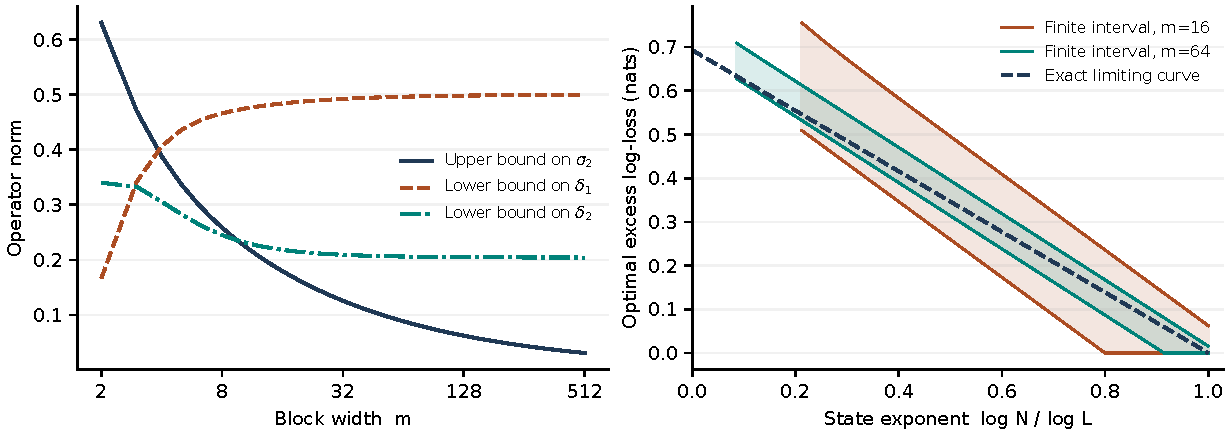
\includegraphics[width=\linewidth]{figures/joint.pdf}
 \caption{Finite certificates for the same proper law. Left: a spectral upper bound and structured lower bounds at \(k=1,2\). Right: finite upper and lower bounds and the exact asymptotic state--log-loss curve, with $k=M=1$. Curves are evaluations of inequalities, not fitted errors.}
 \label{fig:joint}
\end{figure}

\section{A test for black-box planners}\label{sec:test}
Suppose a completed plan \(w\) is the concatenation of every \(m\)-bit block once. Let \(P(w)=p\) for the policy under a fixed problem statement. For any positive \(N\)-state controller, put \(c=\min(1,(N/2^m)^{2^m})\). Observing just whether the emitted trace equals \(w\) gives
\begin{equation}
  \KL(P\Vert Q)\ge
  \begin{cases}
     p\log(p/c)+(1-p)\log((1-p)/(1-c)), &p>c,\\
     0,&p\le c.
  \end{cases} \label{eq:event}
\end{equation}
For \(N=1\) and a balanced word of length \(L\), the exact event cap is \(c=L^L/((L+1)^{L+1}2^L)\). This improves the one-state test by charging termination. A positive bound certifies a statement about every controller in the class without fitting one. Zero means that this event alone is inconclusive.

\paragraph{The gate task.}
There are \(2^m\) numbered gates. To open gate \(j\), the planner emits the \(m\) bits of \(j\), most significant first, using action A for zero and B for one. It must traverse all gates in the specified increasing or decreasing order and stop immediately. An incorrect action fails the task. The prompt supplies this rule and the endpoints. An independent verifier decodes the proposed blocks and compares their integer sequence with the required route. Success is exactly the event in \eqref{eq:event}. This is a deterministic planning task with a unique valid action trace; choosing between alternative successful plans lies outside this evaluation.

\paragraph{Checkpoint and observation.}
We evaluated the pinned four-bit ONNX export of Qwen2.5-0.5B-Instruct \cite{qwen,onnxqwen}. At every step we renormalized its logits over the same three token IDs (space-A, space-B, end-of-message). This defines the measured constrained policy. Teacher forcing scores the complete designated plan including the stop. Conditioning separately at each step differs from conditioning the original language model on the global event of valid syntax. We recorded full-vocabulary scores separately. Nontermination, if present, can be assigned to a cemetery outcome for the binary event test.

\begin{table}[ht]
\centering\small
\caption{Teacher-forced log probabilities in nats. Each target includes the final stop. The last column applies to every proper autonomous one-state controller.}\label{tab:qwen}
\begin{tabular}{rr rr rr r}\toprule
&& \multicolumn{2}{c}{Three-token policy}&\multicolumn{2}{c}{Full vocabulary}&\\
$m$ & Length & Asc. & Desc. & Asc. & Desc. & $\log c_1$\\\midrule
1 & 2 & -0.885 & -6.406 & -10.114 & -14.347 & -3.296 \\
2 & 8 & -12.932 & -11.707 & -21.962 & -20.515 & -8.685 \\
3 & 24 & -36.975 & -32.099 & -49.213 & -43.229 & -20.834 \\
4 & 64 & -72.306 & -63.446 & -88.294 & -78.497 & -49.528 \\
\bottomrule\end{tabular}
\end{table}
On the ascending two-action instance the constrained policy assigned the valid trace probability $0.4127$ (rounded). Its best one-state competitor can assign at most $1/27$. Equation~\eqref{eq:event} gives a floor of $0.7046$ nats, rounded down. The other seven one-state event tests, and all eight tests at budgets two and four, returned zero. None of the eight restricted greedy rollouts solved its instance, as determined by the first mismatch with the verified action sequence, including the stop. The full-vocabulary policy crossed none of the reported caps. A teacher-forced success probability and a greedy success indicator answer different questions.

On the two width-one prompts we also enumerated all completed traces under a three-action horizon. For ascending and descending order, the ratios $\sigma_2/\sigma_1$ were respectively 0.856 and 0.989. In both cases the antisymmetric lower bound was below $\sigma_2$. These checkpoint observations do not establish the spectral separation proved for the constructed law.


\begin{figure}[t]
\centering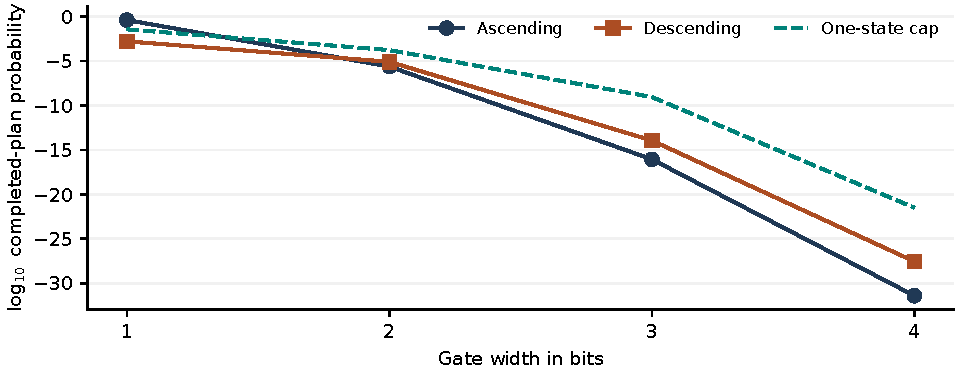
\includegraphics[width=\linewidth]{figures/planner.pdf}
\caption{Log probability of the verifier-accepted action trace under the constrained checkpoint, by gate width and order. The dashed line is the analytic one-state cap; a point above that line certifies positive excess log-loss. Lines between discrete widths guide the eye.}
\label{fig:planner}
\end{figure}

\section{Related work and scope}\label{sec:limits}
Classical realization theory identifies finite rank with linear state dimension \cite{carlyle,fliess}. Singular value automata support spectral truncation under specific guarantees \cite{sva}. Exact spectral-norm approximate minimization is established for one-letter weighted automata \cite{unary}; the multiletter work of Lacroce et al.\ develops a noncommutative formulation \cite{multi}. Our comparison uses the ordinary word-Hankel on counting measure, its concatenation identities and uniform operator norm. Predictive representations use tests of future observations \cite{psr}. Black-box extraction can learn automata from numerical sequence queries \cite{ayache}. Our certificate bounds the error of the entire comparison class. Classical finite-state coding lower bounds \cite{lz} and approximate HMM realization under divergence rate \cite{hmm} supply related viewpoints. We consider the total log-loss on completed finite traces.

The fixed-\(k\) operator example approaches the boundary of stability. The bounds do not quantify approximation on a uniformly stable family, on natural-language text, or for an unrestricted neural architecture with real-valued recurrent state. The KL certificate concerns a declared autonomous finite controller; it gives neither a layer count nor a hardware-byte lower bound for a Transformer or Gated DeltaNet. One quantized checkpoint and eight designed tasks support an audit of the certificate. Broader claims about planning competence would require other tasks, alternative successful trajectories, and more model families.

\paragraph{Code and monograph.}
The DRAGA repository (\href{https://github.com/DatarConsulting/Draga}{\nolinkurl{github.com/DatarConsulting/Draga}}) contains the
\href{https://github.com/DatarConsulting/Draga/blob/main/monograph/monograph.pdf}{companion monograph},
the \href{https://github.com/DatarConsulting/Draga/tree/main/experiments}{experiment code},
and a \href{https://github.com/DatarConsulting/Draga/blob/main/notebooks/DRAGA_Reproduce.ipynb}{reproduction notebook}.
The arXiv ancillary files include the recorded scores and the scripts for scoring the checkpoint and regenerating the figures.

\paragraph{Acknowledgment.}
Generative AI assisted with the construction of the joint example, manuscript drafting, code development, and verification.
\begin{thebibliography}{99}
\bibitem{carlyle} J. W. Carlyle and A. Paz. Realizations by stochastic finite automata. \emph{J. Comput. Syst. Sci.}, 5, 26--40, 1971. \href{https://doi.org/10.1016/S0022-0000(71)80005-3}{doi:10.1016/S0022-0000(71)80005-3}.
\bibitem{fliess} M. Fliess. Matrices de Hankel. \emph{J. Math. Pures Appl.}, 53, 197--222, 1974.
\bibitem{sva} B. Balle, P. Panangaden and D. Precup. Singular value automata and approximate minimization. \emph{Math. Structures Comput. Sci.}, 29, 1444--1478, 2019.
\bibitem{unary} C. Lacroce, B. Balle, P. Panangaden and G. Rabusseau. Optimal approximate minimization of one-letter weighted finite automata. \emph{Math. Structures Comput. Sci.}, 34, 807--833, 2024.
\bibitem{multi} C. Lacroce, P. Panangaden and G. Rabusseau. Towards an AAK theory approach to approximate minimization in the multi-letter case. \href{https://arxiv.org/abs/2206.00172}{arXiv:2206.00172}, 2022.
\bibitem{psr} M. L. Littman, R. S. Sutton and S. Singh. Predictive representations of state. \emph{Advances in Neural Information Processing Systems} 14, 2001.
\bibitem{ayache} S. Ayache, R. Eyraud and N. Goudian. Explaining black boxes on sequential data using weighted automata. \emph{PMLR} 93, 81--103, 2019.
\bibitem{lz} J. Ziv and A. Lempel. Compression of individual sequences via variable-rate coding. \emph{IEEE Trans. Inf. Theory}, 24, 530--536, 1978.
\bibitem{hmm} L. Finesso, A. Grassi and P. Spreij. Approximation of stationary processes by hidden Markov models. \href{https://arxiv.org/abs/math/0606591}{arXiv:math/0606591}.
\bibitem{draga} V. Nobaub. \emph{DRAGA: Dimension Reduction and Guaranteed Approximation. Multiletter Hankel Operators and Executable Memory}. Datar Consulting manuscript, 7 November 2026. Companion monograph, Chapters 1--2.
\bibitem{qwen} Qwen Team. Qwen2.5 technical report. \href{https://arxiv.org/abs/2412.15115}{arXiv:2412.15115}, 2024.
\bibitem{onnxqwen} ONNX Community. \href{https://huggingface.co/onnx-community/Qwen2.5-0.5B-Instruct/tree/22942cb7d7ba4cc81bb4673549ca4d4614469b5e}{Qwen2.5-0.5B-Instruct, ONNX export}, revision \texttt{22942cb7d7ba}, model\_q4.onnx.
\end{thebibliography}

\clearpage
\appendix
\section{Finite operator witnesses}\label{app:op}
The proofs below use the notation of the main text. For an independent reading, \(k\ge1\) is a rank budget, \(m\ge2\), \(K=2^m\), \(L=mK>M>0\), \(r=1-1/m\), \(q=1-r^2\), \(\eta=M/L\), and \(t=(1-\eta)/(1+r)\). All shifts act on counting-measure word space, with inner product linear in the second argument. The direction of a concatenation matters.

\subsection{Decomposing the waiting component}
For \(0\le j\le k\), define \(z_j=\sqrt q\sum_{n\ge0}r^n e_{a^n b^j}\). These unit vectors have disjoint supports. Let \(f(a^n b^k)=qr^n\) and \(f=0\) elsewhere. Thus \(h=f/(1+r)\) is normalized. Sorting the possible cuts before or inside the terminal block gives
\[
 H_f=z_0z_k^*+\sqrt q\sum_{j=0}^{k-1}z_{k-j}e_{b^j}^* .
 \tag{S1}
\]
Indeed a cut in the waiting prefix leaves \(a^i b^k\) on the right, contributing \(qr^{n+i}\) at row \(a^n\). A cut later leaves exactly \(j<k\) copies of \(b\) on the right, contributing \(qr^n\) at row \(a^n b^{k-j}\). The input vectors \((z_k,e_{\ee},\ldots,e_{b^{k-1}})\) are orthonormal, as are the output vectors. Equation (S1) is a singular decomposition with spectrum \(1,\sqrt q,\ldots,\sqrt q\). For any word \(w\), the operator \(H_{\mathbf 1_w}\) maps a suffix basis vector to its complementary prefix, and all other vectors to zero. It is a partial permutation of norm one.

\subsection{An annihilating polynomial respects every continuation}
For a bounded competitor \(G=H_g\) of rank \(s\le k\), let \(V\) be its column space. Write \(c_v[u]=g(uv)\). The right shift \(R_b e_u=e_{ub}\) is isometric, and \(R_b^*c_v=c_{bv}\); hence its restriction \(B=R_b^*|_V\) is a contraction. Multiply its characteristic polynomial by \(z^{k-s}\) and write the result as \(P(z)=z^k+\sum_{j<k}d_jz^j\). Its roots lie in the closed unit disk, so \(|d_j|\le\binom{k}{j}\) and
\[
 S:=\sum_{j<k}|d_j|^2\le \binom{2k}{k}-1.
\]
This also covers \(G=0\) using \(P(z)=z^k\). Apply \(P(B)c_\ee=0\), followed by \(n\) backward right shifts for \(a\). It follows that \(c_{a^n b^k}+\sum_{j<k}d_j c_{a^n b^j}=0\) for each \(n\). Multiplying by \(\sqrt q\,r^n\) and summing in the Hilbert space shows that \(Gx=0\) for \(x=z_k+\sum_{j<k}d_jz_j\). By (S1),
\[
 \|x\|^2=1+S,\qquad \|H_f x\|^2=1+q^2S .
\]
Their squared ratio decreases with \(S\). This gives the structural floor \(\sqrt{(1+(C_k-1)q^2)/C_k}\) for the unnormalized \(H_f\). The argument applies over either field.

For bounded operators, both \(\sigma_2\) (on the compact operators here) and distance to a fixed nonempty subset are 1-Lipschitz in operator norm. Positive scaling commutes with both functions because the structured comparison set is a cone. Now \(H_{p_m}=tH_f+\eta H_{\mathbf1_{w_m}}\), so (S1), the structural floor and the partial permutation estimate prove the finite spectral bounds in Theorem~\ref{th:joint}. In particular, \(\|H_{p_m}\|\to1/2\): the small second singular value is meaningful also relative to the leading one.

\subsection{A sharp limiting constant at rank one}
A nonzero rank-one word-Hankel has a scalar realization \(g(w)=c\prod_{i}x_{w_i}\), with \(c\ne0\). This follows by restricting the backward shifts to its one-dimensional column space; the empty column cannot vanish for a nonzero series. Boundedness forces \(|x_a|^2+|x_b|^2<1\), since its empty column has finite square norm. The row space is spanned by the conjugate of the product sequence. Let \(P\) project onto it and write \(u=|x_a|\), \(v=|x_b|\). For \(k=1\) the absolute normalized overlap of this row with \(z_1\) is at most
\[
 \sqrt q\,\frac{v\sqrt{1-u^2-v^2}}{1-ru}
 \le\sqrt q\,\frac{1-u^2}{2(1-ru)}
 \le\sqrt q .
\]
The first inequality after the fraction maximizes over \(v\); the last uses \(1-u^2\le2(1-u)\le2(1-ru)\). Since \(G(I-P)=0\) and \(H_f^*z_0=z_1\), we have \(\|H_f-G\|\ge\|(I-P)z_1\|\ge\sqrt{1-q}=r\). The zero competitor has error one. Thus \(tr-\eta\le\delta_1(H_{p_m})\le t+\eta\), with both sides tending to \(1/2\). This sharper bound is used in Figure~\ref{fig:joint}.

\paragraph{Sharper constants inherited at other budgets.}
If the boundary limit \(E_{k-1}^{\mathbb F}\) for the unnormalized waiting family is taken from Chapter 1 of \cite{draga}, the same Lipschitz argument gives \(\lim_m\delta_k^{\mathbb F}(H_{p_m})=E_{k-1}^{\mathbb F}/2\). Here \(E_j^{\mathbb F}\) is the distance of \(z^j\) in scalar \(H^2\) to coefficient series of Hankel rank at most \(j\). In particular the resulting limits at budgets two and three are \(\sqrt3/4\) and \(3/8\). The elementary bound above suffices for the simultaneous-separation theorem at every fixed budget. This distinguishes what the present proof establishes independently from the sharper result it inherits.

\section{The positive-state obstruction}\label{app:kl}
For each binary length-\(m\) block \(B\), let \(\psi(B)=\|T_B\|_{\infty\to\infty}\). Since all entries are nonnegative, it is the maximum row sum. With \(T=T_a+T_b\) substochastic,
\[
 \sum_{B\in\{a,b\}^m}\psi(B)\le\sum_{i=1}^N(T^m\mathbf1)_i\le N.
\]
Let \(w=B_1\cdots B_K\) use each block once. The initial distribution has unit \(\ell^1\) norm and \(\|\tau\|_\infty\le1\), whence
\[
 Q(w)\le\prod_{j=1}^K\psi(B_j)
       \le\left(\frac{1}{K}\sum_{j=1}^K\psi(B_j)\right)^K
       \le (N/K)^K .
\]
The middle inequality also holds when some factors vanish. Distinctness of the blocks matters; the argument cannot count \(K\) copies of a single block as distinct resources.

\paragraph{Costs of a rare event.}
For any law \(P\), projecting onto \(\{w\}\) and its complement gives \(\KL(P\Vert Q)\ge d(P(w)\Vert Q(w))\), where \(d\) is binary KL. This is the log-sum inequality applied to the complement. If \(P(w)=\eta\), the weaker but explicit form \(\KL(P\Vert Q)\ge-\eta\log Q(w)-h_2(\eta)\) follows by dropping \(-(1-\eta)\log(1-Q(w))\ge0\). Our word contains \(ba\) for \(m\ge2\), so \(h(w_m)=0\) and \(p_m(w_m)=\eta\). Substituting the cap and \(\eta K=M/m\) proves the KL inequality, uniformly in \(N\). A negative right-hand side can always be replaced by zero.

\paragraph{Finite state cost and exponent.}
Every budget with \(\Ckl_N(p_m)\le\epsilon\) satisfies
\[
 N\ge K\exp\!\left[-\frac mM\{\epsilon+h_2(M/L)\}\right].
 \tag{S2}
\]
The bound survives taking an infimum over controllers. The waiting law is generated by \(k+1\) states: the initial state loops on \(a\) with probability \(r\), enters the \(b\)-chain with probability \(1-r\), and stops after exactly \(k\) copies of \(b\). A deterministic path with \(L+1\) states emits \(w_m\) and stops. An initial distribution on the disjoint union realizes their mixture with \(L+k+2\) states. Since \(\log L=m\log2+\log m\), (S2) and this exact construction prove the exponent-one limit for every vanishing error tolerance. A fixed multiple of \(L\) as a necessary state count would be stronger than this exponent. The proof leaves the subpolynomial factor undetermined.

\paragraph{What happens to the mean?}
The source mean is exactly \((1-\eta)(k+r/(1-r))+M\). Holding \(M\) fixed bounds the exceptional branch's contribution to the mean. It does not bound the mean of the background when \(r\uparrow1\). Changing the mixture background to an empty-word atom would restore a bounded mean but remove the present structured operator witness.

\section{Matching the intermediate state budgets}\label{app:upper}
Partition the lexicographically ordered $m$-blocks into $G=2^\ell$ contiguous groups by their common $\ell$-bit prefix. Each group contains $D=2^{m-\ell}$ blocks. A controller state $(g,j)$ holds the current group and position $j\in\{1,\ldots,m\}$ within its block. When $j\le\ell$ the controller emits bit $j$ of the binary group index. At later positions it chooses a fair bit. It next increments $j$; after position $m$ it stays in the same group with probability $1-1/D$ or advances with probability $1/D$. Advancing past the last group enters one terminal state. This is a time-homogeneous proper generator: each group finishes almost surely, and there are finitely many groups. It has $mG+1$ states and does not receive an external position counter.

One particular trajectory emits the required suffix bits and stays exactly $D$ blocks in each group. Its probability under this generator $U_\ell$ is
\[
 2^{-(m-\ell)K}\left[D^{-1}(1-D^{-1})^{D-1}\right]^G .
\]
For $D=1$ the bracket equals one. For $D>1$, $-(D-1)\log(1-1/D)\le1$ by $\log(1+x)\le x$. Hence
\[
 -\log U_\ell(w_m)\le (m-\ell)K\log 2 + G(\log D+1).
\]
An initial choice between the waiting controller and $U_\ell$ in proportions $1-\eta,\eta$ uses $k+2+mG$ states. On the background support its law dominates $(1-\eta)h$ pointwise. Its contribution to $\KL(p_m\Vert Q)$ there is nonpositive; at $w_m$ it is at most $-\eta\log U_\ell(w_m)$. Since $\eta G=M/(mD)$ and $\log D+1\le D$, the asserted finite upper bound follows.

For $\rho>0$ choose $\ell=\min\{m,\lfloor\log_2((N_m-k-2)/m)\rfloor\}$, which is nonnegative for all sufficiently large $m$. Then $\ell/m\to\rho$. The upper construction and the finite lower bound prove Theorem~\ref{th:frontier}. For $\rho=0$, one can avoid spending $m$ position states. Choose the waiting controller or a single state emitting independent fair letters with stop probability $1/(L+1)$. The latter assigns $w_m$ probability $2^{-L}(L/(L+1))^L/(L+1)$. The resulting $k+2$ state mixture has divergence at most $M\log2+(M/L)(\log(L+1)+1)$, while the lower bound tends to $M\log2$. This proves the endpoint. At $\rho=1$ the first construction gives vanishing divergence even for budgets below $L$ having the same exponent.

As a consequence, for fixed $0<e<M\log2$, the least state budget for $\Ckl_N(p_m)\le e$ has exponent $1-e/(M\log2)$. Indeed (S2) supplies the lower exponent. For any larger exponent strictly less than one, the matching upper limit is strictly below $e$; take the infimum over such exponents. This tradeoff controls total excess log-loss, not log-loss per emitted action.

\section{Transfer to a measured trace probability}\label{app:transfer}
For \(0<p<1\) and \(0<c<p\), the derivative of \(d(p\Vert x)\) with respect to \(x\) is \((x-p)/(x(1-x))<0\) on \(x<p\). This proves the binary event bound after substituting the largest allowed \(x=c\); the complementary case allows \(x=p\). Endpoint conventions follow by continuity. A verified interval \(P(w)\in[p_-,p_+]\) gives the same bound evaluated at \(p_-\) if \(p_->c\), since \(d(p\Vert c)\) increases for \(p>c\). Our empirical evaluations are ordinary floating-point measurements of the exported model; we do not prove forward error bounds for quantized inference.

For a single state, write its stop probability as \(s\) and its conditional letter probabilities as \(u,1-u\). For a balanced length-\(L\) word,
\(Q(w)=s(1-s)^L[u(1-u)]^{L/2}\).
The maximum is attained at \(s=1/(L+1),u=1/2\). This proves the sharp scalar cap, including its termination factor. For example the cap for the two-action plan \(ab\) is \(1/27\), while for a length-64 word listing all four-bit blocks the general four-state cap is \(2^{-32}\). A failure to cross a cap provides no upper bound on the best attainable KL.

\subsection{A finite Hankel check on an observed policy}
A controlled horizon \(T\) defines a different law \(P^{(T)}\): use the three-token policy until it stops or has emitted \(T\) actions, and at that point terminate. Each word of length \(T\) receives the entire mass of its action prefix. With positive support only through \(T\), enumerating every word of lengths \(0\) through \(T\) as both rows and columns yields the whole nonzero part of \(H_{P^{(T)}}\). No arbitrary finite-section extrapolation is involved. The horizon is part of this derived observation law.

Every rank-one scalar word-Hankel equals its transpose, even over the complex field, because letter multiplication commutes. Therefore for a real observed matrix \(H\),
\[
 \delta_1(H)\ge \frac12\|H-H^\top\|_{\op},
 \qquad \delta_1(H)\ge\sigma_2(H).
\]
Indeed transpose preserves operator norm and the triangle inequality applied to \(H-G\) gives the first bound. The same reasoning on the finite block also lower bounds a full-space competitor. The experiment compares the two lower bounds. A skew bound below \(\sigma_2\) cannot witness a structure-induced gap. Exhaustive horizons and incomplete-prefix blocks require distinct interpretations.

\section{Reproducibility and failure cases}\label{app:repro}
The notebook contains the plotting and scoring programs, the measured per-step log probabilities, prompts, and the TeX sources. A default CPU run reconstructs the calculations and figures from these records; a separate switch downloads the pinned model and reruns inference. The model paths, SHA-256 digests and versions are embedded. Figures use analytic inequalities or teacher-forced probabilities and have no fitted parameters. Reported KL values are rounded down when stated as numerical lower bounds at the printed precision.
The action interface uses token IDs 362 (space-A), 425 (space-B), and 151645 (end of message). The ID order and complete chat prompt are checked by the released program. Each model call evaluates the target prefix causally; no search or target-specific logit mask is used. The measured sweep used the CPU execution provider of ONNX Runtime 1.32.0, three intra-operation threads and one inter-operation thread. The measured scoring time, after initializing the session, was 8.6 seconds. Only public model parameters and generated gate instances were used.
\begin{center}
\begin{tabular}{lrrrr}\toprule
Order at $m=1$ & $\sigma_1$ & $\sigma_2$ & $\frac12\|H-H^\top\|$ & Rank-gap witness\\\midrule
Ascending & 0.7037 & 0.6023 & 0.3643 & Inconclusive \\
Descending & 0.6924 & 0.6848 & 0.4594 & Inconclusive \\
\bottomrule\end{tabular}\end{center}


The comparator receives a single problem-dependent initialization and then runs autonomously. Giving it the current gate number or continually rereading the prompt introduces an external information channel. Similarly, the three-token policy can be evaluated by any architecture with next-token scores, while the numerical values reported here belong only to the tested checkpoint and decoding protocol. Truncating the output at three actions serves the separate finite Hankel diagnostic. It is not used to score the long plans.

\end{document}
